\documentclass[oneside]{VUMIFPSkursinis}
\usepackage{algorithmicx}
\usepackage{algorithm}
\usepackage{algpseudocode}
\usepackage{amsfonts}
\usepackage{float}
\usepackage{amsmath}
\usepackage{bm}
\usepackage{caption}
\usepackage{color}
\usepackage{float}
\usepackage{graphicx}
\usepackage{listings}
\usepackage{subfig}
\usepackage{ltablex}
\usepackage{longtable}
\usepackage{wrapfig}
\usepackage{subfig}
\usepackage{pbox}
\renewcommand{\labelenumii}{\theenumii}
\renewcommand{\theenumii}{\theenumi.\arabic{enumii}.}
\renewcommand{\labelenumiii}{\theenumiii}
\renewcommand{\theenumiii}{\theenumii\arabic{enumiii}.}
\newcolumntype{P}[1]{>{\centering\arraybackslash}p{#1}}
\usepackage[%  
    colorlinks=true,
    linkcolor=black
]{hyperref}
\university{Vilniaus universitetas}
\faculty{Matematikos ir informatikos fakultetas}
\department{Programų sistemų katedra}
\papertype{Programų sistemų inžinerija II laboratorinis darbas II}
\title{Reikalavimų analizė ir techninė architektūra}
\titleineng{Requirements Analysis and Technical Architecture}
\status{2 kurso 3 grupės studentai}



\supervisor{Audronė Lupeikienė, M. Darbuot., Dr.}
\date{Vilnius – \the\year}

\bibliography{bibliografija}

\begin{document}
\maketitle
\tableofcontents

\section{Anotacija}

\section{Sistemos detalus projektas}
	\subsection{Sistemos užduotys}
		\subsubsection{Užduočių diagramos}

			\begin{figure}[h]
    				\centering
    				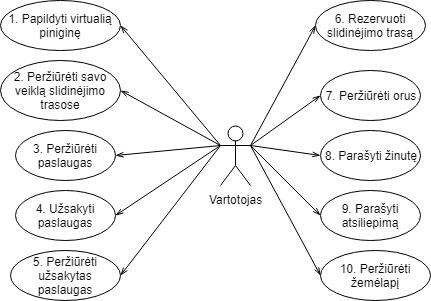
\includegraphics[width=0.75\textwidth]{useCaseVartotojas.png}
    				\caption{Vartotojo užduočių diagrama}
    				\label{fig:VartotojoUseCasel}
			\end{figure}

			\begin{figure}[h]
    				\centering
    				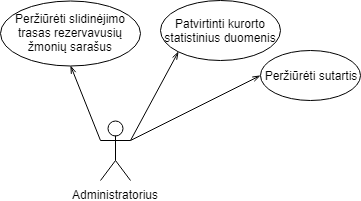
\includegraphics[width=0.75\textwidth]{useCaseAdministratorius.png}
    				\caption{Vartotojo užduočių diagrama}
    				\label{fig:VartotojoUseCasel}
			\end{figure}

		\subsubsection{Robastiškumo diagramos}


			\begin{figure}[h]
    				\centering
    				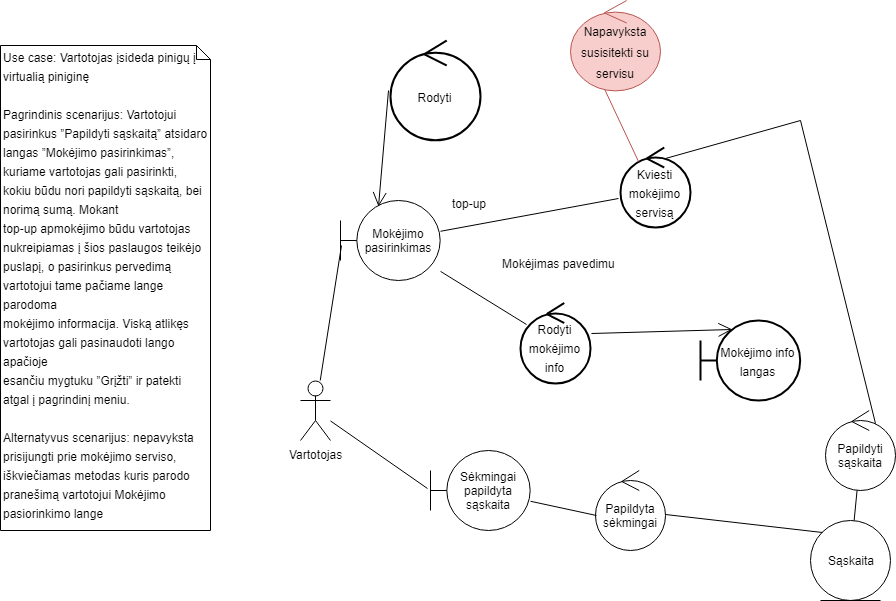
\includegraphics[width=0.75\textwidth]{rob1.png}
    				\caption{Vartotojo užduočių diagrama}
    				\label{fig:VartotojoUseCasel}
			\end{figure}

			\begin{figure}[h]
    				\centering
    				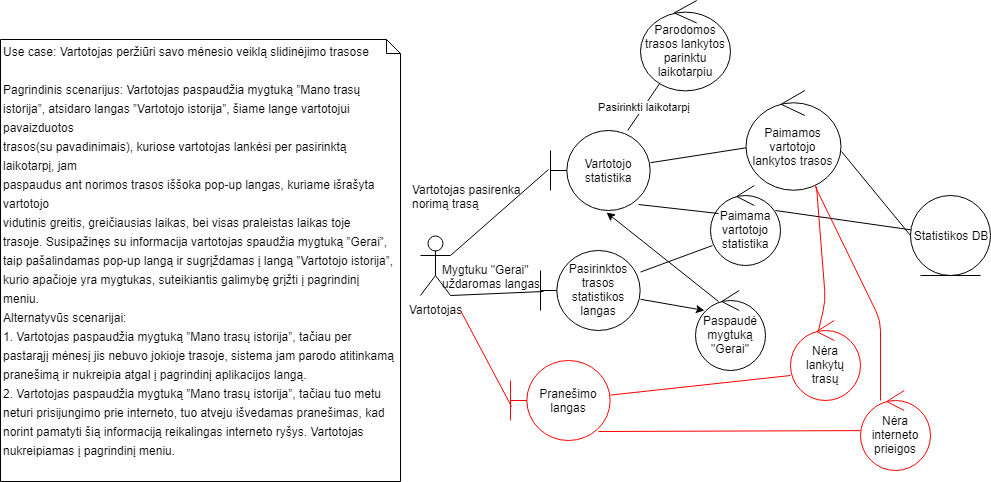
\includegraphics[width=0.75\textwidth]{rob2.png}
    				\caption{Vartotojo užduočių diagrama}
    				\label{fig:VartotojoUseCasel}
			\end{figure}

			\begin{figure}[h]
    				\centering
    				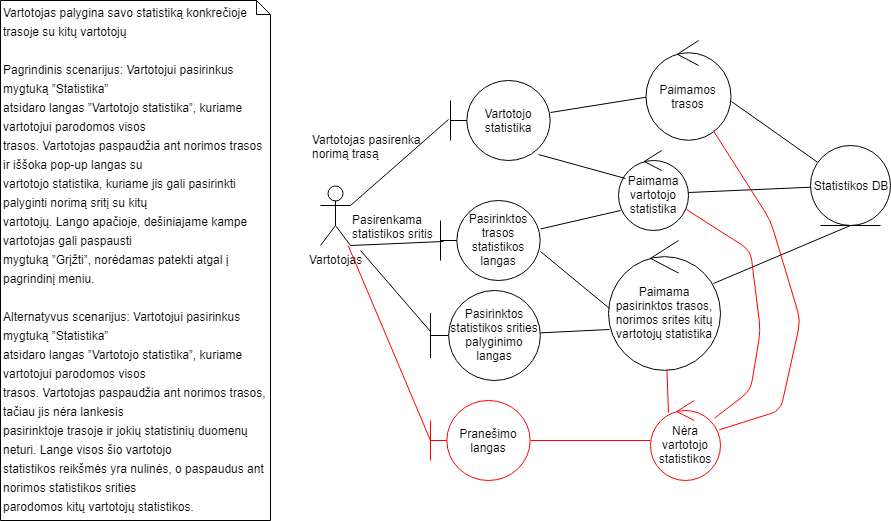
\includegraphics[width=0.75\textwidth]{rob3.png}
    				\caption{Vartotojo užduočių diagrama}
    				\label{fig:VartotojoUseCasel}
			\end{figure}

			\begin{figure}[h]
    				\centering
    				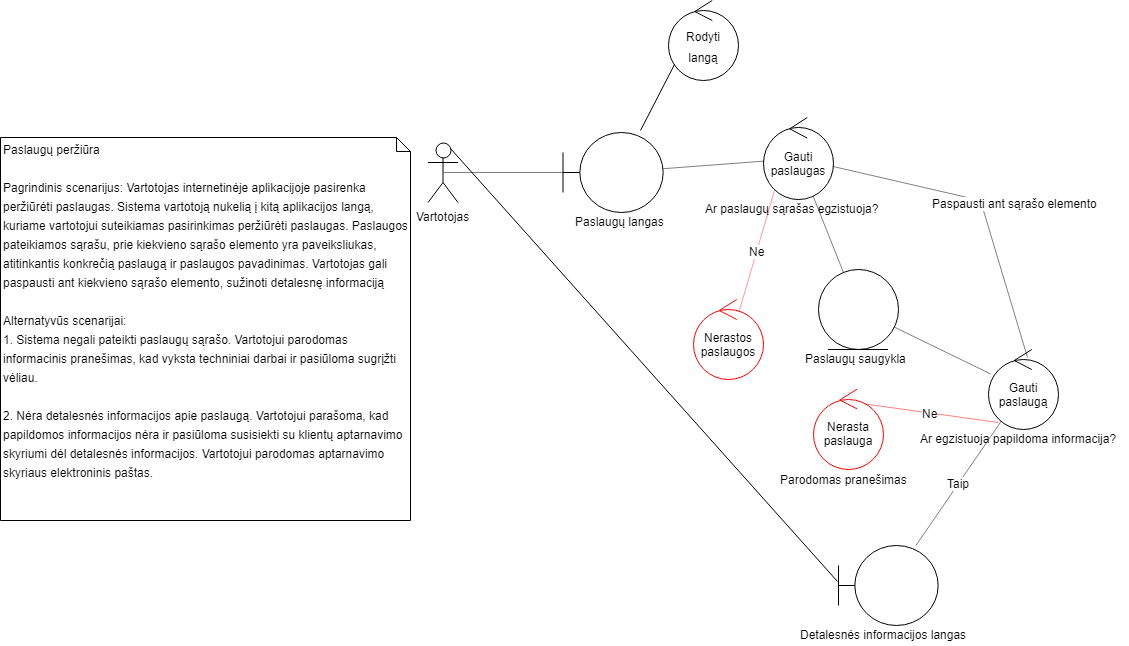
\includegraphics[width=0.75\textwidth]{rob4.png}
    				\caption{Vartotojo užduočių diagrama}
    				\label{fig:VartotojoUseCasel}
			\end{figure}

			\begin{figure}[h]
    				\centering
    				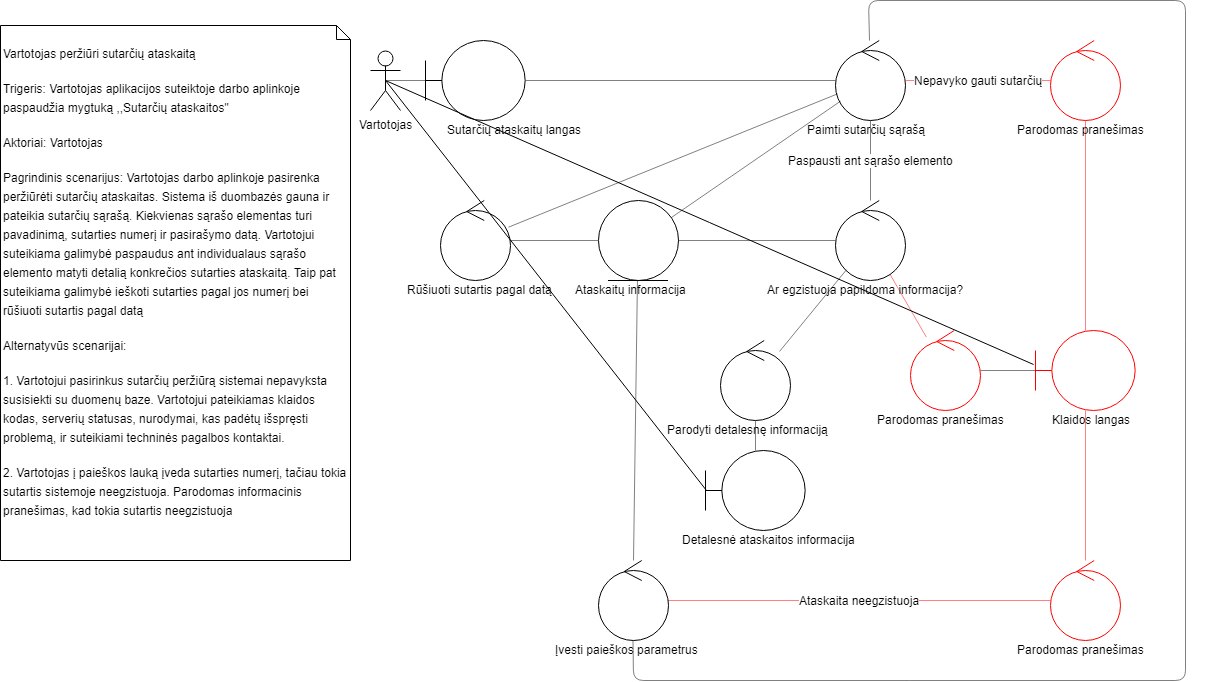
\includegraphics[width=0.75\textwidth]{rob5.png}
    				\caption{Vartotojo užduočių diagrama}
    				\label{fig:VartotojoUseCasel}
			\end{figure}

			\begin{figure}[h]
    				\centering
    				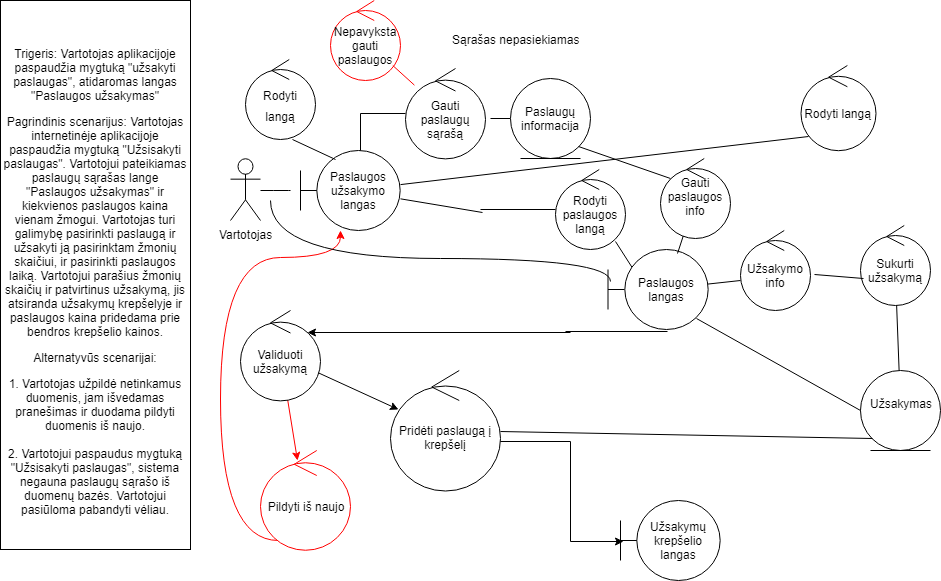
\includegraphics[width=0.75\textwidth]{rob6.png}
    				\caption{Vartotojo užduočių diagrama}
    				\label{fig:VartotojoUseCasel}
			\end{figure}

			\begin{figure}[h]
    				\centering
    				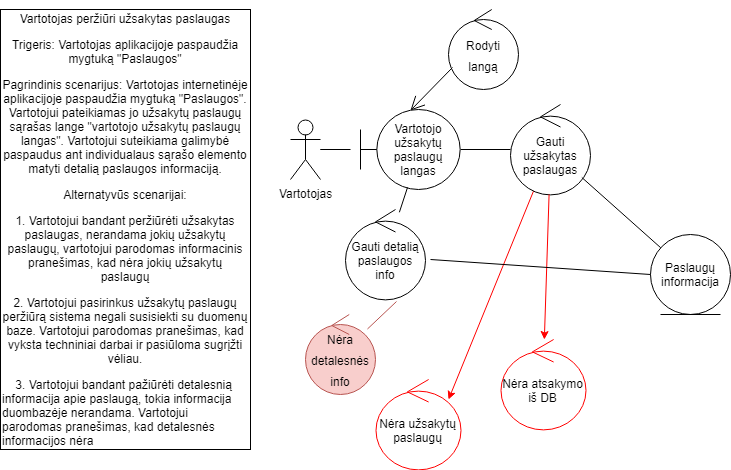
\includegraphics[width=0.75\textwidth]{rob7.png}
    				\caption{Vartotojo užduočių diagrama}
    				\label{fig:VartotojoUseCasel}
			\end{figure}

			\begin{figure}[h]
    				\centering
    				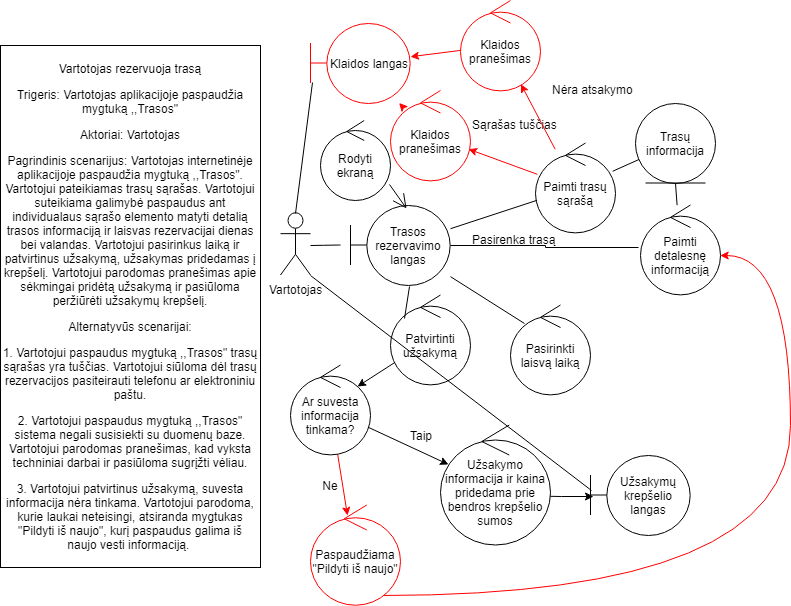
\includegraphics[width=0.75\textwidth]{rob8.png}
    				\caption{Vartotojo užduočių diagrama}
    				\label{fig:VartotojoUseCasel}
			\end{figure}

			\begin{figure}[h]
    				\centering
    				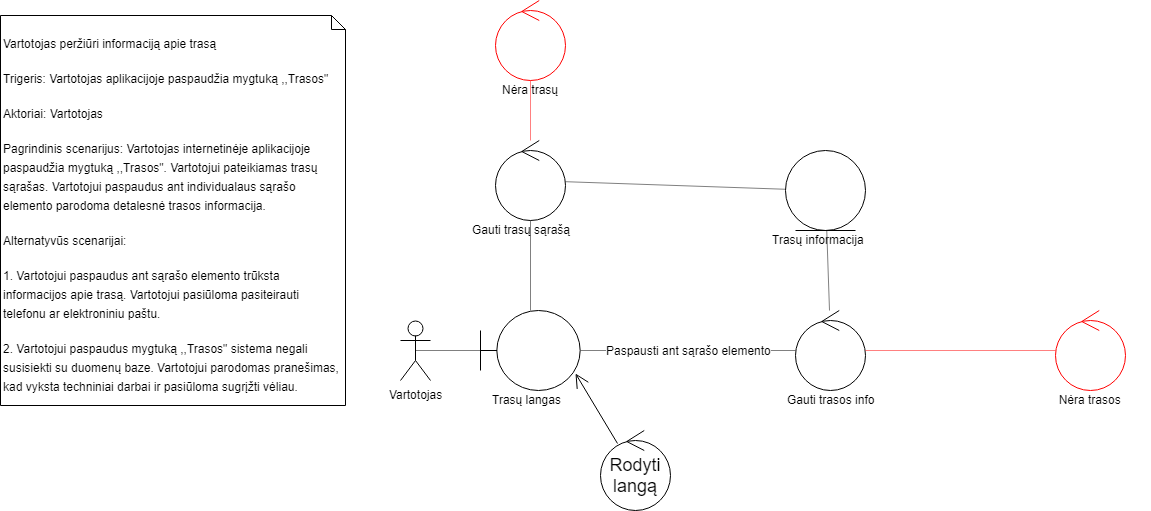
\includegraphics[width=0.75\textwidth]{rob9.png}
    				\caption{Vartotojo užduočių diagrama}
    				\label{fig:VartotojoUseCasel}
			\end{figure}

			\begin{figure}[h]
    				\centering
    				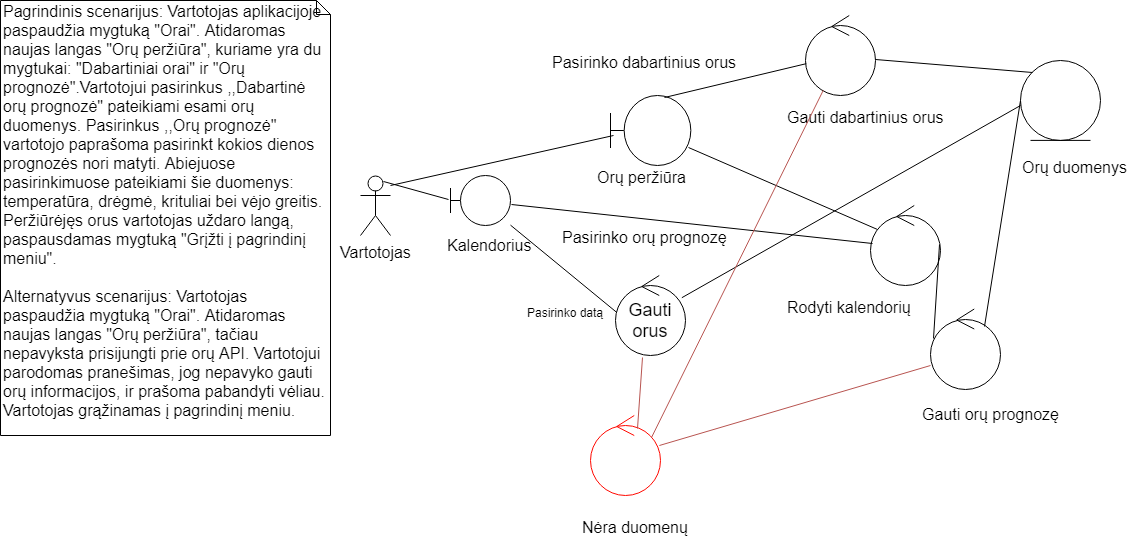
\includegraphics[width=0.75\textwidth]{rob10.png}
    				\caption{Vartotojo užduočių diagrama}
    				\label{fig:VartotojoUseCasel}
			\end{figure}

			\begin{figure}[h]
    				\centering
    				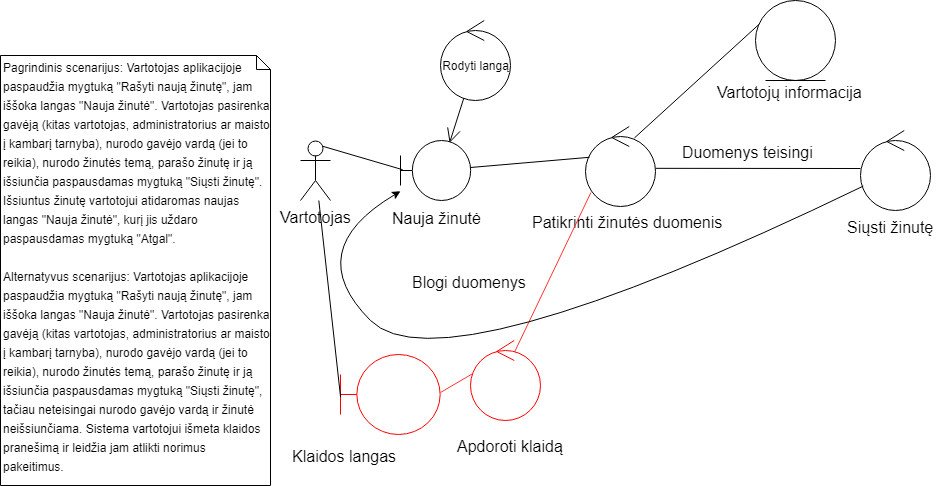
\includegraphics[width=0.75\textwidth]{rob11.png}
    				\caption{Vartotojo užduočių diagrama}
    				\label{fig:VartotojoUseCasel}
			\end{figure}

			\begin{figure}[h]
    				\centering
    				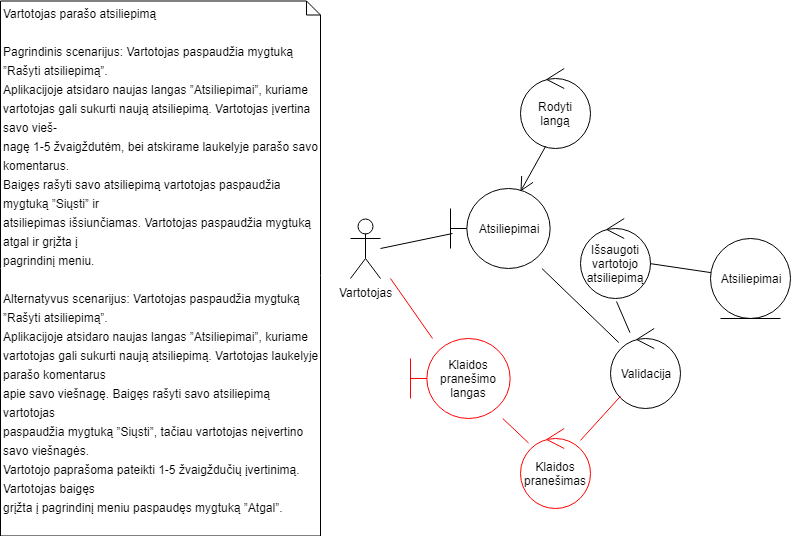
\includegraphics[width=0.75\textwidth]{rob12.png}
    				\caption{Vartotojo užduočių diagrama}
    				\label{fig:VartotojoUseCasel}
			\end{figure}

			\begin{figure}[h]
    				\centering
    				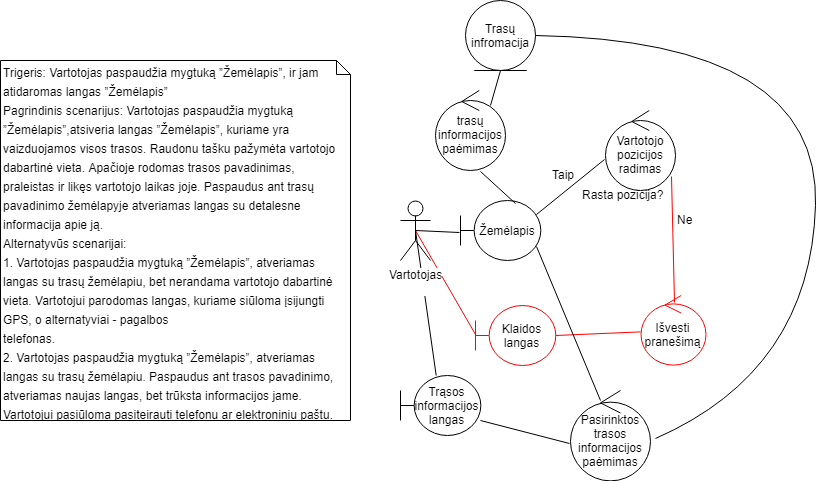
\includegraphics[width=0.75\textwidth]{rob13.png}
    				\caption{Vartotojo užduočių diagrama}
    				\label{fig:VartotojoUseCasel}
			\end{figure}

			\begin{figure}[h]
    				\centering
    				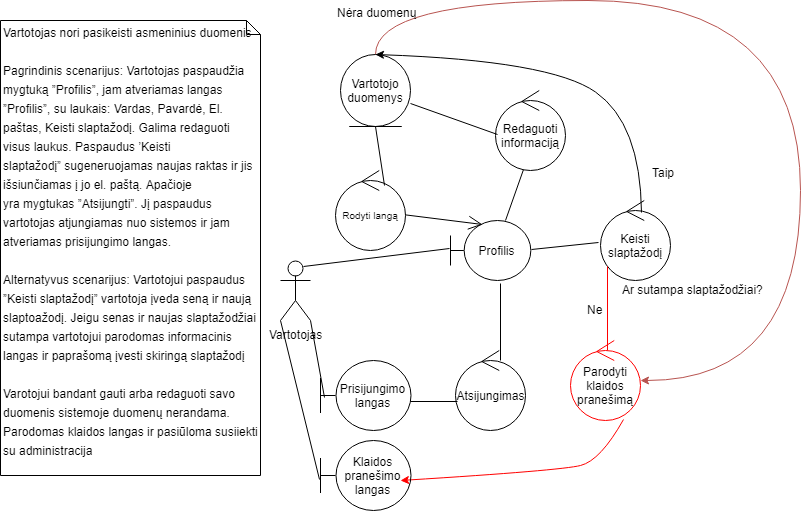
\includegraphics[width=0.75\textwidth]{rob14.png}
    				\caption{Vartotojo užduočių diagrama}
    				\label{fig:VartotojoUseCasel}
			\end{figure}


		\subsubsection{Sekų diagramos}
	\subsection{Sistemos struktūra}
		\subsubsection{Klasių diagrama}
	

\section{Detalaus projekto peržiūra}
	\subsection{Peržiūra}
	\subsection{Atsekamumas}

\section{Testavimo planas ir scenarijai}
	\subsection{Programinių vienetų testai}
	\subsection{Sistemos užduočių testai}

\section{Sistemos techninė architektūra}
	\subsection{Sistemos komponentų diagrama(galutinė pataisyta)}
	\subsection{Išdėstymo diagrama(galutinė pataisyta)}




\section{Sistemos realizacija}
	\subsection{Duomenų bazės schema}
	\subsection{Pradiniai programų kodai ir aprašas}


\end{document}